% Name: Closure of a braid
% Description: The braid σ₁³ with each top end joined to the bottom end in the same position, which closes it up into the trefoil knot.
% Tags: braid closure, trefoil, Alexander's theorem, knot

\usetikzlibrary{braids}

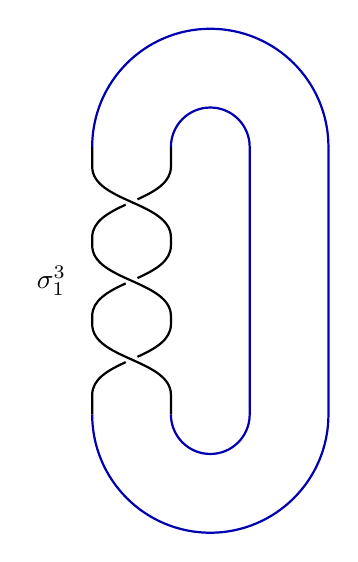
\begin{tikzpicture}[thick]
  \pic[braid/.cd, every strand/.style={thick}, border height=2mm] (b) {braid={s_1 s_1 s_1}};
  % the inner end closes with radius 0.5, the outer one with radius 1.5, so the loops nest
  \draw[blue!70!black] (b-2-s) arc[start angle=180, end angle=0, radius=0.5] coordinate (p)
    -- (p |- b-rev-2-e) arc[start angle=0, end angle=-180, radius=0.5];
  \draw[blue!70!black] (b-1-s) arc[start angle=180, end angle=0, radius=1.5] coordinate (q)
    -- (q |- b-rev-1-e) arc[start angle=0, end angle=-180, radius=1.5];
  \node[left=2mm] at (b.west) {$\sigma_1^3$};
\end{tikzpicture}
